\section{\iflanguage{english}{Previous Work}{Frühere Arbeiten}}
This section summarizes previous and related work from selected papers.

In 2008 Volkov and Demmel examined in \cite{Volkov2008} the characteristics of 
back than recent NVIDIA \acp{GPU}\footnote{GeForce 8, 9 and 200 series} using 
microbenchmarks. Based on their findings they present beside other linear 
algebra algorithms a parallel \ac{GEMM} algorithm.
% Here Volkov uses the CUDA term "vector length" which is a synonym for the 
% size of a work-group in OpenCL.
% Furthermore work-groups are called gangs in CUDA.
To increase the performance of \ac{GEMM} they propose the use of as small 
work-groups as possible, ``to avoid the extra costs associated with spreading 
the data across many warps'' \cite[Section 2.2]{Volkov2008}. They recommend 
placing data in registers than in shared memory because the register file is 
larger and higher in the memory hierarchy than shared memory \cite[Section 
2.3]{Volkov2008}. They found that the kernel launch overhead back than was 
\SIrange{3}{7}{\micro\second} for asynchronous and 
\SIrange{10}{14}{\micro\second} for synchronous invocation. They measured 
that the timing of data transfer of up to \SI{100}{\mega\byte} between 
\acs{CPU} and \acs{GPU} via a \acs{PCIe} 1.1 $\times$16 interface can be 
modeled as given in \cref{eq:pciPortTiming}.
\begin{equation}
 \label{eq:pciPortTiming}
 \text{Time} = \text{\SIrange{10}{17}{\micro\second}} + \frac{\text{bytes 
transferred}}{\text{\SIrange{2.2}{3.4}{\giga\byte\per\second}}}
\end{equation}
The application of a pointer chasing algorithm revealed the features of the 
memory system like latency and structure \cite[Section 3.3]{Volkov2008}. 
Pipeline latency has been measured by taking the time it takes executing a 
large set of dependent operations like $a = a * b + c$. From the results they 
conclude the number of instruction streams necessary to hide this latency 
\cite[Section 3.4]{Volkov2008}.

Volkov and Demmel present a \ac{GEMM} algorithm in that works 
as follows. The result matrix $C$ is partitioned into blocks of $64 \times 16$ 
elements. Each block is calculated by a work-group of 64 work items. They 
consider only matrix sizes that are multiples of the block size and matrices 
stored in column-major layout. Per step the work items load a $16 \times 16$ 
block collaborative from $B$ and each work item loads 16 elements of a row of 
$A$ and then updates one row of the $64 \times 16$ block. In the end each 
work item stores its 16 results in $C$ \cite[Section 4]{Volkov2008}. An OpenCL 
version of this algorithm is given in \cref{lst:volkov2008}.
\lstinputlisting[caption={GEMM algorithm by Volkov and Demmel implemented in 
OpenCL},label={lst:volkov2008},language=OpenCL]{sources/volkov_2008.cl}



Lai and Seznec presented in 2013 in \cite{Lai2013} an approach to estimate the 
performance upper 
bound for \ac{GPU} applications based on the algorithm used and analysis on 
assembly code level. They used their results to optimize a \ac{SGEMM} 
completely in assembler level by hand for NVIDIA Fermi and Kepler 
\acp{GPU}\footnote{GeForce 500 and 600 series}. 
Their finding is that \ac{SGEMM} can at maximum achieve \SI{82.5}{\percent} of 
the peak performance on Fermi and \SI{57.6}{\percent} on Kepler \acp{GPU}.

They use the considerations and optimizations given in the following with which 
they achieve \SI{74.2}{\percent} of the peak performance on Fermi \ac{GPU} and 
\SI{44.5}{\percent} of the peak performance on Kepler \ac{GPU}. Due to the 
nature of computing devices not all instructions have a counterpart in the 
mathematical algorithm they represent. These ``auxiliary instructions'' 
\cite[Section 4.1]{Lai2013} should be minimized. They reveal that the 
throughput 
reaches its maximum if there are 5 times more math instructions than 
``auxiliary instructions'' \cite[Figure 2]{Lai2013}. With this ratio they found 
that the number of active work items should be at least 512 on Fermi \ac{GPU} 
and 1024 on Kepler \ac{GPU} to get close to the best throughput. On assembly 
level they optimize as follows. They allocate for each work item only the 
maximal number of registers available per work item such that all data stays in 
the registers and does not get spilled out. They reorder instructions such that 
dependent instructions are interleaved by other instructions.

Lai and Seznec introduce the formula in \cref{eq:potentialPeakPerformance} to 
calculate the potential peak performance.
\begin{align}
\label{eq:potentialPeakPerformance}
P_{potential} &= min(P_{MemBound},P_{SMBound}) \\
P_{SMBound} &= \frac{B_R^2}{B_R^2 + B_R * 2 * F_I} * F_T * P_{theoretical} \\
P_{MemBound} &= \frac{2 * B_{Sh}^2 * \#{GlobalMem\_bandwidth}}{2 * B_{Sh} * 4} 
\\
B_{Sh} &= \sqrt{T_B * B_R^2} \\
F_I &= f(B_R, \text{choice of LDS instruction})
\end{align}
\begin{multline}
F_T = f(B_R,\text{\# dispatch units},\text{\# streaming processors},\\ 
    \text{\# load/store units}, \text{\# active threads}) 
\end{multline}

$B_R$ is the register blocking factor. $T_B$ is the number of work items 
per block of the result matrix $C$. They retrieve the throughput factor $F_T$ 
and the instruction factor $F_I$ by experiment.



In \cite{Djinevski2013} from 2013 Djinevski et al. showed that it is possible 
to achieve superlinear speedup for matrix multiplication on \acp{GPU} using the 
cache hierarchy. Their idea is to store (parts of) the matrix $B$ in the L2 
cache such that all cores can share the data. Each core handles a submatrix of 
$A$. The code reconstructed from the description given in their paper is given 
in \cref{lst:djinevski2013}. 

\lstinputlisting[caption={\ac{GEMM} algorithm by 
Djinevski et al. implemented in OpenCL},label={lst:djinevski2013}, 
language=OpenCL]{sources/djinevski_2013.cl}

\subsection{Evaluation of Muesli in the Context of Autotuning OpenCL 
versions of \acs{GEMM}}

The \ac{Muesli} is a C++ library that provides common, 
configurable patterns and (distributed) data structures for data and task 
parallel programming. The library is implemented in terms of the \ac{MPI}.

There are three different distributed data structures. Their names are 
\texttt{DistributedArray}, \texttt{DistributedMatrix} and 
\texttt{DistributedSparseMatrix}. Each of which is templatized such that it 
is capable of holding any value type. They all provide so called skeletons as 
member functions that transform the data stored according to a function 
specified by the programmer. This is the same orthogonal concept as in the 
\ac{STL} of C++ where functions like \texttt{std::transform} apply a function 
in some specific manner to all elements of a range. The key difference is that 
\ac{Muesli} offers to the programmer a \textit{global} view of the whole data 
structure while it internally decomposes it into partitions that are assigned 
to individual processes (\textit{local} view). This is completely transparent 
to the programmer \cite[Chapter 3.1]{Ciechanowicz2009}.

Task parallelism is modeled in \ac{Muesli} by a system of processes that 
communicate via streams of data ``by nesting and combining predefined process 
topologies'' like \texttt{DivideAndConquer} or \texttt{BranchAndBound} 
respectively. Inside these strategies atomic building blocks are responsible 
for transforming the data streams \cite[Chapter 4]{Ciechanowicz2009}. Four such 
atomic 
building blocks are predefined by the library. \texttt{Initial} and 
\texttt{Final} model the source and sink of a data stream. \texttt{Atomic} 
represents a task that generates one output per input, while \texttt{Filter} 
generates an arbitrary number of output values per input value, including zero 
outputs \cite[Chapter 4.1]{Ciechanowicz2009}.

The \ac{GEMM} algorithm can be parallelized in several ways. For each element 
of the result matrix $C$ a dot product of the order of the 
inner dimension of both operands $A$ and $B$ has to be carried out (data 
parallelism). The dot product involves multiplying corresponding elements of 
the rows of $A$ and the columns of $B$ (task parallelism). 
\cref{lst:MuesliGEMM} demonstrates how \ac{GEMM} can be implemented using 
\ac{Muesli}. On the task parallel site there is used a pipeline that first 
decomposes the matrices $A$ and $B$ into rows resp. columns. In the second stage 
all pairs of rows and columns are generated. In the next step they are 
multiplied and then summed up. At last the results are stored in $C$. During 
multiplication and summation the code relies on data parallelism.

Splitting up summation and multiplication is reasonable in this case as there 
is no \texttt{zipWithInPlaceFold} function. It would be possible to mimic the 
same behavior using \texttt{mapIndexInPlaceFold} or 
\texttt{mapIndexInPlaceScan} but that would require using partial application 
to have access to the elements of the other vector. For an OpenCL 
implementation on \ac{GEMM} one should not split summation and addition as 
these can make use of the MAD hardware instruction.

In general the matrices of an application are stored using the same memory 
layout. Common layouts are row- and column-major layouts. When carrying out a 
matrix multiplication the elements of at least one operand will not be accessed 
sequentially. As cache lines store chunks of data there will be many cache 
misses. Therefor the \texttt{Farm} approach used here which generates arrays of 
contiguous memory locations is quite interesting. Then the operand in question 
can be accessed once to bring its elements in a contiguous order. If the data 
isn't required to outlive the execution of the \ac{GEMM} algorithm this 
swapping can be done in place, thus saving memory.

Distributing data over several processes is inherent to OpenCL even though it 
is not that transparent as in \ac{Muesli}.

\lstinputlisting[caption={\ac{GEMM} algorithm implemented using 
\ac{Muesli}},label={lst:MuesliGEMM},language=C++]{sources/gemm_in_muesli.cpp}

\subsection{Evaluation of clMAGMA in the Context of Autotuning \acs{GEMM}}

clMAGMA\footnote{http://icl.cs.utk.edu/magma/index.html} is an open source 
library for high performance \ac{DLA} computing on heterogeneous systems. The 
library provides algorithms compatible to the \ac{BLAS} standard. To guarantee 
cross-platform performance portability its strategy is to rely on the vendors' 
highly optimized math routines like \ac{GEMM} as can be found in e.\,g. 
AMD's clMath \footnote{\url{http://developer.amd.com/%
tools-and-sdks/heterogeneous-computing/amd%
-accelerated-parallel-processing-math-libraries/}} or Intel's 
\ac{MKL}\footnote{https://software.intel.com/en-us/intel-mkl}. On top of that 
clMAGMA implements its logic and scheduling system to make use of all computing 
resources of a system \cite{Dongarra2013}.

Nevertheless the authors of the clMAGMA project propose several 
different \ac{GEMM} implementations, even autotuned ones.

In \cite{Li2009} from 2009 the authors use the \ac{GEMM} kernel presented in 
\cite{Volkov2008} as a template for their auto-tuning system that has a code 
generator and a heuristical search engine. In the end they outperform 
\cite{Volkov2008} by more than a quarter. In total they have six parameters to 
vary the kernels generated, namely the block sizes, the work-group size and a 
parameter that specifies the layout of the blocks loaded into shared memory.

In 2010 a \ac{GEMM} is proposed in \cite{Nath2010} that makes use of the then 
newly introduced memory hierarchy for \acp{GPU}. The involved matrices are 
still loaded blockwise but they are first loaded to shared memory and then to 
registers. Back then they achieved \SI{58}{\percent} of the peak performance.
Note that changes in the architecture may not be captured by the auto-tuners 
such that new generations of \ac{GPU} may also require change the auto-tuners 
as well.
In a later paper that year the same authors present the so called 
\textit{pointer redirecting} technique to further accelerate \ac{DLA} kernels. 
This technique deals with the problem that arises if the matrices' dimensions 
are not an integer multiple of the blocking factors. If workers try to access 
elements beyond the dimensions of the operands they are forced to use the 
elements of the outer most column resp. row \cite[Section 3]{Nath2010a}. 
Besides that the pointer redirecting algorithm does not consume extra memory 
nor involves extra copying as well as initializing the extra elements it 
performs better for smaller and comparable for larger matrix dimensions 
\cite[Section 5]{Nath2010a}.

In \cite{Kurzak2011} from 2011 autotuning of CUDA \ac{GEMM} kernels is 
presented. The \ac{GEMM} is shown is striclty compliant to the \ac{BLAS} 
standard and follows the convention that each work group calculates one block 
of the result matrix $C$ in several iterations loading blocks of $A$ and $B$ in 
each step. The work group size and its shape as well as the sizes of the the 
respective blocks are parameterized such that a kernel generator can produce a 
large set of kernels. The kernels are checked against several criteria such 
as hardware constraints \cite[Section 5.3]{Kurzak2011}. All kernels are then 
executed and the fastest ones are kept.


\subsection{Evaluation of \acs{FloPoCo} in the Context of Autotuning \acs{GEMM}}
\ac{FloPoCo} is an open source framework written in C++ for the generation of 
arithmetic datapaths in VHDL. It ships with a command line executable that 
generates synthesizable VHDL code according to a mathematical function specified 
by the user and a given target device.

The example given in \cref{lst:flopocoExample} will produce VHDL code for a
floating-point adder with ten bits of exponent and 36 bits of mantissa running 
on a Xilinx Virtex4 at \SI{200}{\mega\hertz}.
\ac{FloPoCo} supports various devices and the framework abstracts their 
characteristics in a class called \texttt{Target}. This is helps in supporting 
many different devices and in being future-proof as new models appear 
frequently. The same holds true for OpenCL compute devices. Thus knowledge 
about the devices should be used for generating the kernel code.

FloPoCo is even capable of generating code for more complex datapaths such as 
the one specified in \cref{lst:complexDatapth}.

\begin{lstlisting}[language=bash,caption={Exemplary invocation of the 
\acs{FloPoCo} code generator},label={lst:flopocoExample}]
flopoco -target=Virtex4 -frequency=200 FPAdder 10 36
\end{lstlisting}

\begin{lstlisting}[language=bash,caption={Pseudo program for a more complex 
datapath},label={lst:complexDatapth}]
R = X*X + Y*Y + Z*Z;
output R;
\end{lstlisting}

As depicted in the example no actual information about how to implement the 
plus and multiply operators are given. Often there is more than one possible 
implementation and these are available via a class hierarchy in \ac{FloPoCo} as 
in \cref{fig:flopocoOperators}. This gives the freedom to vary several 
equivalent implementations. In the OpenCL programming language there are 
several equivalent constructs that may perform differently depending on the 
underlying hardware. In \cite[Section 6.8.7.5]{AMD2013} it is mentioned that 
\texttt{for}, \texttt{do} and \texttt{while} loops can produce code that 
performs differently. In addition OpenCL provides special expressions that may 
make use of specialized hardware. Examples are given in 
\cref{lst:openclInstructions}. Thus it is worth varying these instructions in a 
kernel generator.

\begin{lstlisting}[language=OpenCL,caption={Selected OpenCL instructions and 
their semantic},label={lst:openclInstructions}]
 d = fma( a, b, c );    // d = a * b + c;
 w = select( x, y, z ); // w = z ? x : y;
 u = dot( v1, v2 );     // u = v1.x * v2.x + ... + v1.w * v2.w;
\end{lstlisting}


\begin{figure}[htbp]
 \centering
 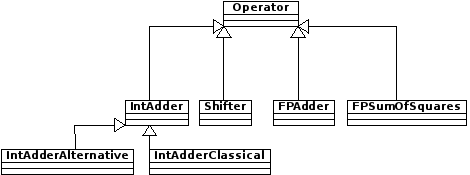
\includegraphics{flopocoClassHierarchy}
 \caption{Extract of the \acs{FloPoCo} class hierarchy}
 \label{fig:flopocoOperators}
\end{figure}


